% \chapter*{\Huge Big Title Here}
% \addcontentsline{toc}{chapter}{Big Title Here}  % Add to TOC if needed

\chapter{Structural synergism is bovine respiratory disease modelling} % Main chapter title


%----------------------------------------------------------------------------------------
%	SECTION 
%----------------------------------------------------------------------------------------
\section{Introduction}
%-----------%-----------
%	SOUS-SECTION 
%-----------%-----------
\subsection{Elements of context}

%-----------
%	SOUS-SOUS-SECTION 
%------------
\begin{itemize}
    \item In our previous work, we showed ... but there has been more recently published models, more realistic as they differentiate the specific effects of pathogens, one for Mh, BRSV and Mh. "Multiple experts is better than one average expert". 

\end{itemize}


\subsection{Article originality}

\begin{itemize}
    \item  In this chapter we propose a method for distinguishing and identifying the most livelily mechanistic model using observations whenever there are multiple valid representation of knowledge. (give more detail on the distinguishability side). Distinguishing pathogen amongsth ...
    \item A model is only as good as the quality of it's decisions. In this chapter, we also prove that choosing the expert to prognoses a disease yields benefits. (give more detail on the informed-decision)
\end{itemize}


%-----------%-----------
%	SOUS-SECTION 
%-----------%-----------
\subsection{Main contributions and perspectives}

\begin{itemize}
    \item  We proposed method for numerically distinguishing BRD mechanistic models using the dynamics of symptomatic with a 95\% average accuracy. This
    \item We showed that relying on pathogen-informed decisions to administer antibiotic treatments can  yield benefits compared to conventional decisions rules. Reducing Antimicrobial usage by 44\% constantly across various batch configurations, while preserving the financial benefit. The findings of this work could contribute against antimicrobial resistance and public health.
\end{itemize}

Up to now, we have shown how deep learning be automate the diagnosis of BRD at punctual date points , this is affordable for most deep learning models as it requires less data training (achieve 72‰ accuracy with less 30 videos of training). We have also shown a mechanistic model for BRD can be parameterised to fit reliable diagnosis at punctual data points in order to prognose and explicit the dynamics of BRD at a larger temporal resolution.  Through this new chapter, we handled the case when they are multiple valid expertise almost like for human when you have a doctor generalist but also multiple experts (surgeon, dentist, opthamologist, ...), how to could you choose the most likely model for optimal decision-making. 

We showed deep learning is the expert for diagnosis using sensor observations, epidemiological mechanistic model are the expert for long-term predictions at larger temporal resolution. However to make relevant recommendations, we need a mixture of experts diagnosis and prognosis using contextual observations. The bottleneck of chaining two methods which are experts at their objective is how to handle the proxy linking both ? In the next chapter, we show how to sketch a coupling methodology between a deep learning and an epidemiological mechanistic model.



\subsection{[In French] Résumé grand public}



%-----------------------------------
%	SECTION 
%-----------------------------------
\section{Peer-reviewed preprint in bioarxiv, 2025}


    % \input{chapters/chap1-article} # pas besoin de mettre un file appart sauf si j'ai des choses spécifiques à rajouter pour cette partie
    \includepdf[pages=-]{articles/article3.pdf}  % Replace with your actual filename
    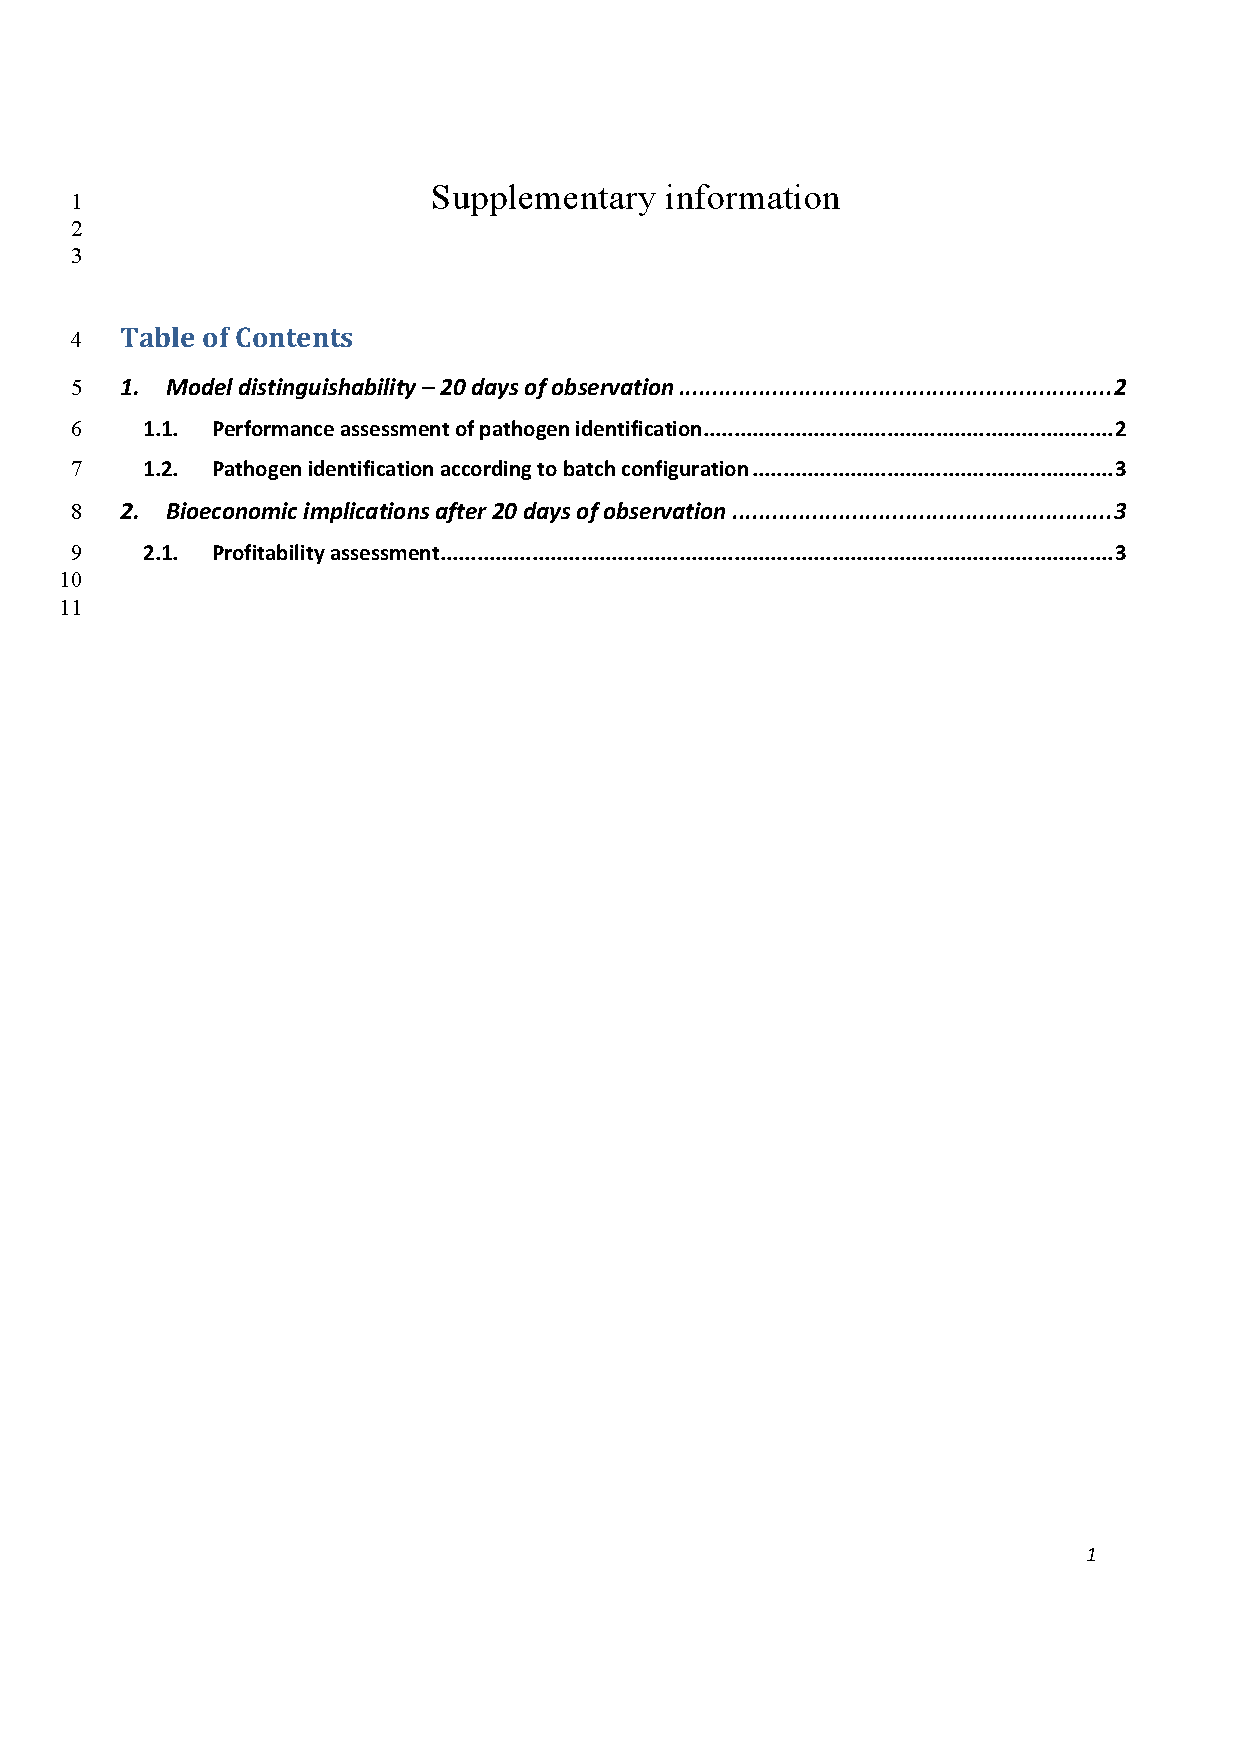
\includepdf[pages=-]{articles/supp-mat3.pdf}
